\begin{center}
	\bigskip \bigskip
	{\huge \bf Appendix} \\
	\bigskip
\end{center}
\addcontentsline{toc}{section}{Appendix}

\section{Appendix A}
\label{appendix-runes}
\subsection*{Rune Table}
\begin{table}[ht]
	\centering
	{\renewcommand{\arraystretch}{1.5}
		\begin{tabular}{ | c | c | p{5.5cm} | p{7cm} | }
			\hline
			\textbf{Rune} & \textbf{Name} & \textbf{Meanings} &
			\textbf{In-game function} \\
			\hline
			\raisebox{-0.25\totalheight}{
\includegraphics[width=0.45cm]{pictures/runes/algiz.png}} &
			Algiz & \small Elk, Defencs, Protection & \small Build Tower \\
			\hline
			\raisebox{-0.25\totalheight}{
\includegraphics[width=0.45cm]{pictures/runes/berkanan.png}} &
			Berkanan & \small Birch, Birth, Earth & \small Element: Earth \\
			\hline
			\raisebox{-0.25\totalheight}{
\includegraphics[width=0.45cm]{pictures/runes/dagaz.png}} &
			Dagaz & \small Day, Light, Balance & \small Element: Light \\
			\hline
			\raisebox{-0.25\totalheight}{
\includegraphics[width=0.45cm]{pictures/runes/ehwaz.png}} &
			Ehwaz & \small Horse, Movement, Speed & \small Tower: Attackspeed \\
			\hline
			\raisebox{-0.5\totalheight}{
\includegraphics[width=0.45cm]{pictures/runes/fehu.png}} &
			Fehu & \small Cattle, Wealth, Dynamic Property & \small Farm: Cow Upgrade \\
			\hline
			\raisebox{-0.5\totalheight}{
\includegraphics[width=0.45cm]{pictures/runes/gebo.png}} &
			Gebo & \small Gift, Trade & \small Tower: Money On Hit, Village: Damage costs Money \\
			\hline
			\raisebox{-0.25\totalheight}{
\includegraphics[width=0.45cm]{pictures/runes/haglaz.png}} &
			Haglaz & \small Winter, Widespread Destruction & \small Tower: Splash Damage \\
			\hline
			\raisebox{-0.25\totalheight}{
\includegraphics[width=0.45cm]{pictures/runes/ingwaz.png}} &
			Ingwaz & \small Wine, Growth & \small Farm: Wine Upgrade \\
			\hline
			\raisebox{-0.25\totalheight}{
\includegraphics[width=0.45cm]{pictures/runes/iwaz.png}} &
			Ihwaz & \small Link & \small Tower: Enable multiple different Elements \\
			\hline
			\raisebox{-0.25\totalheight}{
\includegraphics[width=0.45cm]{pictures/runes/isaz.png}} &
			Isa & \small Ice, Freeze, Isolation & \small Tower: Slow On Hit \\
			\hline
			\raisebox{-0.25\totalheight}{
\includegraphics[width=0.45cm]{pictures/runes/jeran.png}} &
			Jera & \small Harvest, Circle of Life & \small Build Farm \\
			\hline
			\raisebox{-0.25\totalheight}{
\includegraphics[width=0.45cm]{pictures/runes/kauna.png}} &
			Kenaz & \small Fire, Torch, Ignition & \small Element: Fire \\
			\hline
			\raisebox{-0.25\totalheight}{
\includegraphics[width=0.45cm]{pictures/runes/laukaz.png}} &
			Laukaz & \small Water, River, Tears & \small Element: Water \\
			\hline
		\end{tabular}
	}
	\caption{Rune table for runes 1-14}
\end{table}


\begin{table}[H]
	\centering
	{\renewcommand{\arraystretch}{1.5}
		\begin{tabular}{ | c | c | p{5cm} | p{7cm} | }
			\hline
			\textbf{Rune} & \textbf{Name} & \textbf{Meanings} &
			\textbf{In-game function} \\
			\hline
			\raisebox{-0.5\totalheight}{
\includegraphics[width=0.45cm]{pictures/runes/mannaz.png}} &
			Mannaz & \small Human, Community, Intelligence & \small Build Village \\
			\hline
			\raisebox{-0.5\totalheight}{
\includegraphics[width=0.45cm]{pictures/runes/naudiz.png}} &
			Naudhiz & \small Distress, Hardship & \small Village: Villager defend Village, Tower: temp. SpeedUpgrade \\
			\hline
			\raisebox{-0.5\totalheight}{
\includegraphics[width=0.45cm]{pictures/runes/othalan.png}} &
			Othanal & \small Heritage, Wealth, Static Property & \small Village: inc. Money Capacity, Tower: Money on Kill \\
			\hline
			\raisebox{-0.25\totalheight}{
\includegraphics[width=0.45cm]{pictures/runes/pertho.png}} &
			Perthro & \small Luck, Destiny, Random & \small Random Upgrade Rune \\
			\hline
			\raisebox{-0.25\totalheight}{
\includegraphics[width=0.45cm]{pictures/runes/raido.png}} &
			Raido & Travel, Path & Build Path: obsolete \\
			\hline
			\raisebox{-0.5\totalheight}{
\includegraphics[width=0.45cm]{pictures/runes/sowilo.png}} &
			Sowilo & \small Sun, Warmth, targeted Power & \small Tower: Beam Upgrade, Farm: Sunflower Upgrade \\
			\hline
			\raisebox{-0.25\totalheight}{
\includegraphics[width=0.45cm]{pictures/runes/thurisaz.png}} &
			Thurisaz & \small Giant, Thorns, Defense & \small Tower: AOE around Tower\\
			\hline
			\raisebox{-0.25\totalheight}{
\includegraphics[width=0.45cm]{pictures/runes/tiwaz.png}} &
			Tiwaz & \small Sky, Honor, Discipline & \small Element: Air\\
			\hline
			\raisebox{-0.25\totalheight}{
\includegraphics[width=0.45cm]{pictures/runes/uruz.png}} &
			Uruz & \small Healing, Health  & \small Farm: Upgrade, Village: inc. max. HP\\
			\hline
			\raisebox{-0.5\totalheight}{
\includegraphics[width=0.45cm]{pictures/runes/wunjo.png}} &
			Wunjo & \small Happiness, Harmony & \small Multiple Elements, Farm: Upgrade for Sunflowerfarm \\
			
			\hline
		\end{tabular}
	}
	\caption{Rune table for runes 15-24}
\end{table}


\clearpage
\pagebreak
\section{Appendix B}
\label{appendix-illustrations}

\subsection*{Illustrations}

Illustrations as found in~\cite{kraemer-oppidum-maching}.

\begin{figure}[ht]
	\centering
	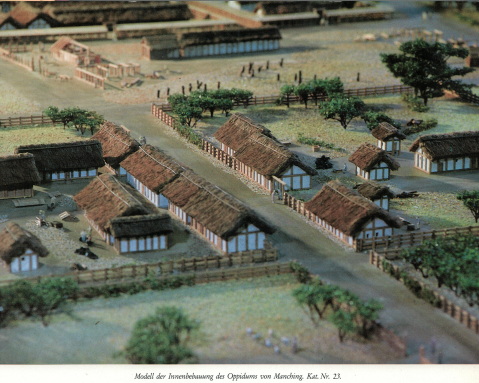
\includegraphics[width=\linewidth]{pictures/scan_manching_2.png}
	\caption{Model of the inner buildings of the  Oppodium of Manching.}
\end{figure}

\begin{figure}[ht]
	\centering
	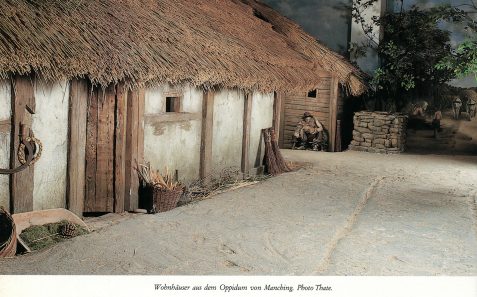
\includegraphics[width=\linewidth]{pictures/scan_manching_1.png}
	\caption{A illustration of a living house.}
\end{figure}

\begin{figure}[ht]
	\centering
	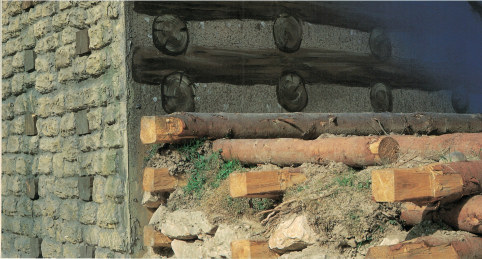
\includegraphics[width=\linewidth]{pictures/scan_manching_4.png}
	\caption{Construction of a wall.}
\end{figure}


\begin{figure}[ht]
	\centering
	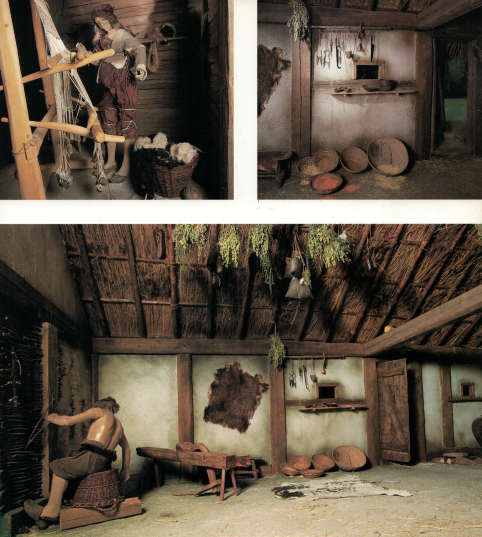
\includegraphics[width=\linewidth]{pictures/scan_manching_3.png}
	\caption{Inner view of a living house.}
\end{figure}

\clearpage
\pagebreak
Illustrations from Rieckhoff and Biel's \textit{'Die Kelten in Deutschland`}~\cite{rieckhoff-walls1}\cite{rieckhoff-walls2}\cite{rieckhoff-tower}.

\begin{figure}[ht]
	\centering
	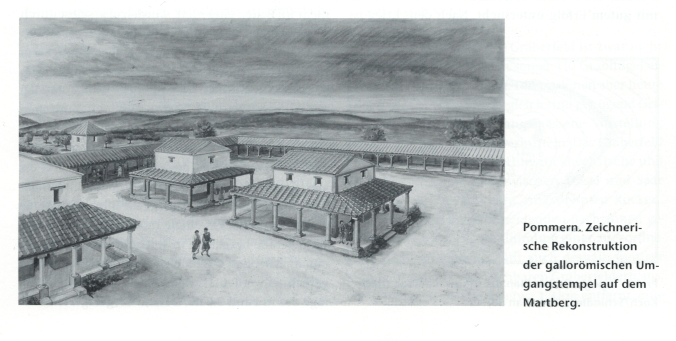
\includegraphics[width=\linewidth]{pictures/scan_rieckhoff_tower.png}
	\caption{We modeled our tower after the tower on the left of the background.}
\end{figure}

\begin{figure}[ht]
	\centering
	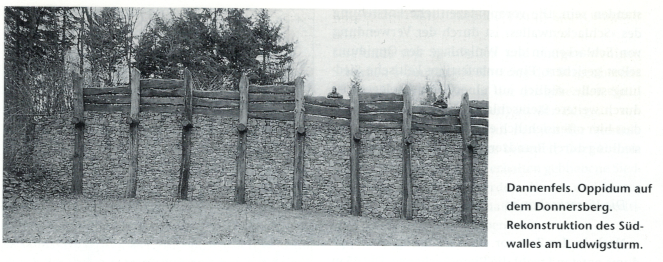
\includegraphics[width=\linewidth]{pictures/scan_rieckhoff_wall1.png}
	\caption{Reconstruction of a Oppidum wall.}
\end{figure}

\begin{figure}[ht]
	\centering
	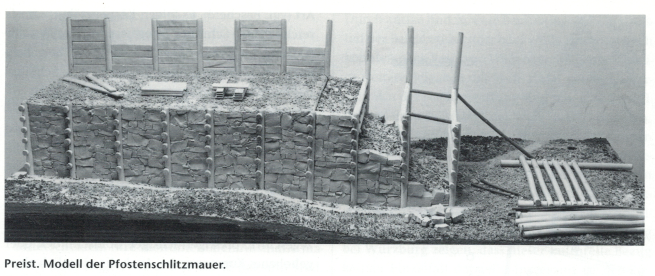
\includegraphics[width=\linewidth]{pictures/scan_rieckhoff_wall2.png}
	\caption{Another reconstruction of an Oppidum wall.}
\end{figure}

\begin{figure}[ht]
	\centering
	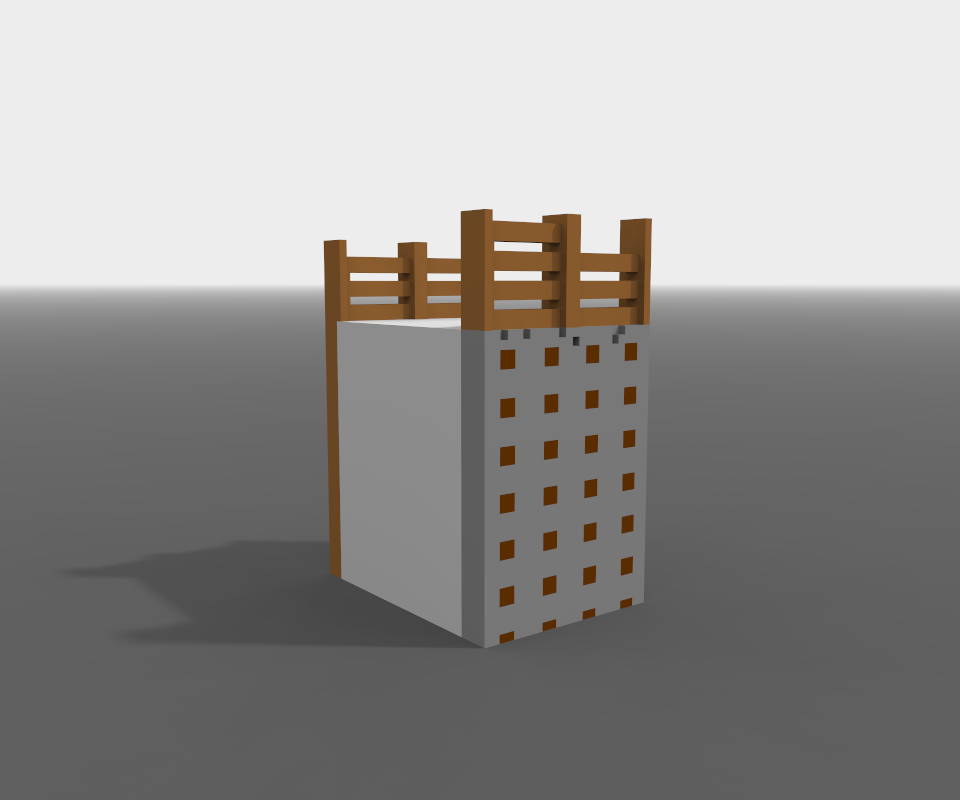
\includegraphics[width=\linewidth]{pictures/stone_wall.png}
	\caption{Our stone wall model.}
\end{figure}


\clearpage
\pagebreak
\vspace*{-3.5cm}
\section{Appendix C}
\label{appendix-userstudy}

Raw test results.

\begin{figure}[H]
	\centering
	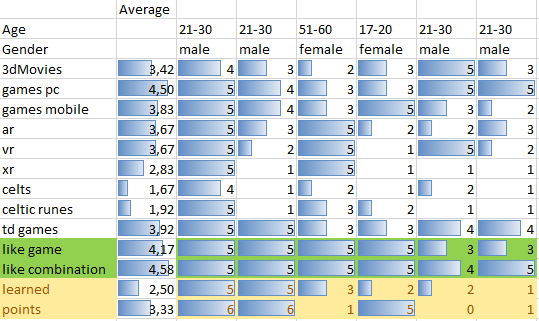
\includegraphics[width=0.95\linewidth]{figures/test-results1.png}
	\caption{Test results 1-6.}
	\label{fig:test-result1}
\end{figure}

\begin{figure}[H]
	\centering
	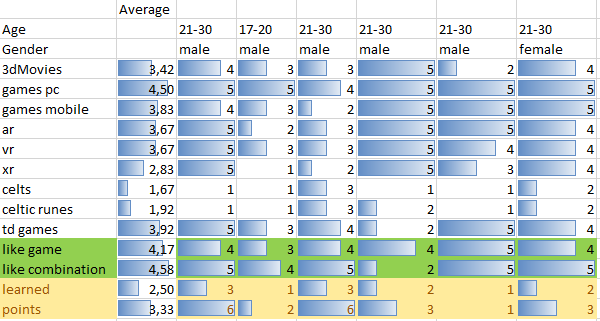
\includegraphics[width=0.95\linewidth]{figures/test-results2.png}
	\caption{Test results 7-12}
		\label{fig:test-result1}
\end{figure}


